\documentclass[10pt,twocolumn]{article}

\usepackage[a4paper,top=17mm,bottom=19mm,left=17mm,right=17mm,columnsep=7mm]{geometry}
\usepackage{amsmath}
\usepackage{booktabs}
\usepackage{graphicx}
\usepackage{microtype}
\usepackage{tabularx}
\usepackage{enumitem}
\usepackage{xcolor}
\usepackage[hidelinks]{hyperref}
\usepackage{fancyhdr}
\usepackage{balance}

\definecolor{btlblue}{HTML}{172B4D}
\definecolor{btlrule}{HTML}{B9C2CF}
\definecolor{btlshade}{HTML}{F3F5F8}
\definecolor{btlgreen}{HTML}{197D6D}

\setlength{\parindent}{1em}
\setlength{\parskip}{0pt}
\setlist{nosep,leftmargin=*}
\renewcommand{\familydefault}{\rmdefault}
\renewcommand{\arraystretch}{1.08}
\hypersetup{colorlinks=true,linkcolor=btlblue,urlcolor=btlgreen,citecolor=btlblue}

\pagestyle{fancy}
\fancyhf{}
\fancyhead[L]{\footnotesize BAD THEORY LABS}
\fancyhead[R]{\footnotesize Behavior Before Perplexity}
\fancyfoot[C]{\footnotesize\thepage}
\renewcommand{\headrulewidth}{0.3pt}

\newcommand{\model}{BTL-3 Compact}
\newcommand{\code}[1]{\texttt{#1}}
\newcommand{\tightcaption}[1]{\vspace{-1mm}\caption{#1}\vspace{-2mm}}

\begin{document}

\twocolumn[
\begin{center}
{\LARGE\bfseries\color{btlblue} Behavior Before Perplexity}\par
\vspace{2mm}
{\large A failure-driven recipe for compressing a 27B agentic model to 8.39 GB}\par
\vspace{4mm}
{\normalsize Bad Theory Labs}\par
{\small July 2026}\par
\end{center}

\begin{minipage}{0.90\textwidth}
\small
\textbf{Abstract.}
We set out to make BTL-3, a 27B coding and tool-use model, small enough for local deployment. The first candidates looked acceptable under reconstruction loss, perplexity, and teacher-forced token agreement, yet could not make a valid tool call. We therefore changed the unit of optimization from a tensor to a deployed behavior. The resulting build uses a sequential affine-lattice vector core, measured INT4 and BF16 precision islands, a rank-8 behavior correction, a selectively rescued embedding, and a rank-32 output-head correction. The final native GGUF is 8,392,369,600 bytes and contains 2,416 byte-verified tensor payloads. On a newly authored private tool-contract gate, the full-precision teacher solved 90 of 100 turns and the compact artifact retained 83 of those 90. This is 92.2\% conditional retention overall, with 100\% retention on single, parallel, sequential, and abstention cases, but only 30\% on parallel-multiple calls. We describe the failed routes, the exact recipe that survived, and the limits of the claim. The contribution is the selection and proof procedure, not a claim to have invented vector quantization, LDLQ, mixed precision, or LoRA.
\end{minipage}
\vspace{6mm}
]

\section{What we built}

\model{} is the compact edition of the frozen BTL-3 checkpoint. It keeps the complete 64-layer text decoder and the model's 262,144-token architectural context. It removes the vision tower and optional speculative head. The release file is a GGUF, but stock GGUF tensor types are not sufficient for its AVQ2 representation; execution uses the packed CUDA and Metal operators in the BTL llama.cpp backend.

The file size is 8.39 decimal GB, or 7.82 GiB. This number includes the decoder, embeddings, output head, adapter, scales, codebooks, metadata, and alignment. It is not the size of a decoder-only experiment. The final SHA-256 is:

\begin{quote}\small\ttfamily
2ddf9527620a17a2a6739d184a7096c4\\
5712092e6589128792ec6254e94dc30c
\end{quote}

We use ``retention'' narrowly. The reported 92.2\% is conditional tool-contract retention on one private gate. It is not 92.2\% of general intelligence, coding ability, or benchmark score.

\section{Why the ordinary metrics failed}

The project began with binary and ternary targets. Those targets were attractive because their storage arithmetic was clean. Their behavior was not.

A complete 0.8B ternary proxy was mechanically valid at 1.7177 bits per weight. Its perplexity increased by 9.75 times, none of seven teacher-passed tool cases survived, and executable code fell from 2/6 to 0/6. A later 4B experiment was more deceptive: a recovered magnitude-initialized model reached 34\% assistant-token agreement while producing zero valid actionable calls. It rambled to the token limit and received accidental credit on irrelevance because a model that cannot call a tool also cannot make an irrelevant call.

SparseGPT initialization made the 4B model less dead. At equal sparsity, block-Hessian reconstruction reduced pre-training KL by 63\% relative to magnitude thresholding and raised top-1 agreement from 3.5\% to 26.6\%. After 300 recovery steps it was the only low-bit variant that emitted any valid tool calls. It was still not useful: simple calls reached 28\%, parallel calls remained at 0\%, and 60\% of generations failed to stop.

This changed our release rule. Perplexity, KL, token agreement, and local reconstruction error remained useful diagnostics. None could promote a candidate. Promotion required free-running behavior from the exact packed prefix or artifact.

\begin{table}[t]
\centering
\small
\caption{Negative controls that changed the recipe.}
\begin{tabularx}{\columnwidth}{@{}Xrr@{}}
\toprule
Candidate & Token proxy & Action result \\
\midrule
0.8B ternary & 43.8\% top-1 & 0/7 tools \\
4B magnitude recovery & 34.0\% top-1 & 0\% calls \\
4B SparseGPT recovery & 65.5\% top-1 & partial only \\
Scalar GGUF pair & complete file & 27/63 retained \\
\bottomrule
\end{tabularx}
\end{table}

\section{The recipe}

The final method grew out of the failed controls. It is easiest to reproduce as an ordered procedure. Changing that order changes the method.

\subsection{Freeze the source and split the data}

We pinned the Qwen3.6-27B source and frozen BTL-3 adapter checksum before calibration. Evaluation cases were excluded by ID, source ID, content hash, tool name, and family. The base revision was:

\begin{quote}\footnotesize\ttfamily
6a9e13bd6fc8f0983b9b99948120bc37\\
f49c13e9
\end{quote}

The core UniSVQ gate used 256 reconstruction rows and 128 source-disjoint validation rows. Half of each split was broad code or frontend material and half was agent/tool material. The agent half was balanced across single, sequential, parallel, parallel-multiple, and abstention behavior. This replaced an earlier category-sorted calibration file whose first rows were almost entirely single calls and which produced misleadingly strong early gates.

The layer-8 MLP capture contained 294,544 training tokens and 178,952 validation tokens. Later release packing used a smaller restart-safe operating set only after the representation and behavioral ladder had already passed.

\subsection{Collect the state the packed model will actually see}

For layer $\ell$, we ran the calibration sequences through layers $0,\ldots,\ell-1$ using the already packed prefix. We captured the resulting input $X_\ell$ and accumulated the full second moment in FP64,
\begin{equation}
H_\ell = \frac{1}{N}X_\ell^\top X_\ell.
\end{equation}
We recorded centered-covariance diagnostics but used the full second moment for the executed path. Calibrating every layer from full-precision hidden states was rejected because later layers would then be fitted to inputs they never receive at inference time.

\subsection{Fit the four-weight affine lattice}

Compatible matrices were divided into 128-wide blocks. A seeded randomized Hadamard transform was applied on the input and output block axes. Consecutive groups of four transformed weights were represented by one four-dimensional affine integer lattice code. The executed configuration was:

\begin{itemize}
\item vector size 4 and block size 128;
\item an affine $4\times4$ lattice map initialized from an orthogonal basis;
\item block-LDLQ assignment with propagated quantization error;
\item ten coordinate-refinement passes;
\item scale candidates 0.8, 1.0, and 1.2 times the initial scale;
\item exact two-bit packed codes plus counted affine metadata.
\end{itemize}

For a block with transformed weight $W'$ and curvature $H$, assignment minimized the curvature-weighted error
\begin{equation}
\mathcal{L}_{\mathrm{block}} = \mathrm{tr}\!\left((W'-\widehat W')H(W'-\widehat W')^\top\right).
\end{equation}
LDLQ propagated the error of each assigned four-weight group into the remaining groups. This is the material difference from independent nearest-code rounding.

\subsection{Treat a gated MLP as one unit}

Qwen's MLP is not three unrelated matrices:
\begin{equation}
y = W_{\mathrm{down}}\left(\mathrm{SiLU}(W_{\mathrm{gate}}x)\odot W_{\mathrm{up}}x\right).
\end{equation}
We therefore fitted \code{up\_proj}, \code{gate\_proj}, and \code{down\_proj} together when a prefix failure localized to an MLP. The exact layer-8 replacement occupied 66,846,888 bytes at 2.000005 effective bits per weight. Its curvature-weighted relative output MSEs were 0.03420, 0.03004, and 0.02496 for up, gate, and down projections.

We also tested fixed-code affine reconstruction of the three-matrix block. Validation was checked every ten steps with patience three. It stopped at step 170, improving normalized MLP MSE only from 0.090695 to 0.090392. Token agreement fell and KL worsened. We kept the raw PTQ artifact. This rejected an intuitively appealing stage rather than quietly including it in the recipe.

\section{Behavioral bisection}

The first AVQ2 candidate was healthy through eight layers and failed by sixteen. The aggregate token metrics did not locate the cause, so we replayed nested packed prefixes.

Prefixes 9, 10, 12, and 14 all lost the same sequential case that prefix 8 retained. At prefix 9, restoring layer 8's linear-attention projections to BF16 did not recover the case. Restoring the full layer-8 MLP did. The MLP override had worse token metrics than the attention override, yet it was behaviorally correct.

The faithful affine-lattice replacement for that MLP then restored all 24 teacher-correct diagnostic cases, including the lost sequential case. When combined with the old layers 9 through 15, retention fell back to 23/24. There was a second cumulative failure. We repeated the same prefix and module-override procedure instead of starting an unbounded 64-layer run.

The rule used throughout the remainder was:

\begin{enumerate}
\item replay nested prefixes until a behavior first changes;
\item override one module or interacting module group;
\item retain an override only if the same emitted behavior is restored;
\item price the intervention in physical bytes;
\item install it, replay the prefix, and capture fresh downstream activations.
\end{enumerate}

This produced the precision map. It was not assigned by a rule such as ``attention at four bits, MLP at two.''

\section{The final decoder allocation}

The complete source decoder contained 336 AVQ2 vector matrices, 64 group-128 affine INT4 matrices on full-attention paths, one measured AVQ2-to-INT4 island, and 14 behavior-proven BF16 islands. The explicit INT4 island was layer 9 \code{linear\_attn.in\_proj\_z}; promoting it cost 8,601,344 bytes and reduced relative weight MSE to 0.010437.

The BF16 islands were concentrated in layers 10 through 16, with later islands at layers 33 and 36. They covered selected linear-attention input/output projections, attention output/value projections, MLP gates, and MLP down projections. This pattern is a record of observed cliffs, not a general claim about Qwen sensitivity.

Once the vocabulary cost was known, we re-opened only the byte ledger. Two BF16 islands were demoted to group-128 INT4: layer 13 \code{linear\_attn.in\_proj\_qkv} and layer 33 \code{linear\_attn.in\_proj\_z}. They recovered 123,863,040 bytes. The release therefore retains 12 physical BF16 islands. No other decoder allocation changed after the sealed release gate was opened.

\begin{table}[t]
\centering
\small
\caption{The two final byte exchanges.}
\begin{tabularx}{\columnwidth}{@{}Xrr@{}}
\toprule
Tensor & BF16 & INT4 \\
\midrule
L13 in-proj QKV & 104.86 MB & 27.44 MB \\
L33 in-proj Z & 62.91 MB & 16.47 MB \\
\midrule
Recovered & \multicolumn{2}{r}{123.86 MB} \\
\bottomrule
\end{tabularx}
\end{table}

\section{Repair on the deployed graph}

At 64 layers the packed model still knew the tool language, but it over-abstained. We froze every packed weight and trained a correction on the exact compressed forward graph. The final correction is rank-8 LoRA with alpha 16, no dropout, AdamW betas $(0.9,0.95)$, zero weight decay, gradient norm 1.0, sequence length 1,024, and 100 optimizer steps in the saved state. Labels cover assistant tokens only.

The adapter is restricted to layers 40 through 63 and to four module families: \code{linear\_attn.in\_proj\_z}, \code{linear\_attn.out\_proj}, \code{self\_attn.o\_proj}, and \code{mlp.down\_proj}. Training pools explicitly separate abstention, single, sequential, parallel, and parallel-multiple examples. The adapter is not merged into the low-bit codes; the packed matmul and low-rank path are composed at runtime. Its counted payload is 32,440,320 bytes.

On the development gate, the repaired artifact retained 62/63 teacher-correct turns. The unrepaired scalar GGUF route had retained 27/63. Because the 63-turn gate guided engineering choices, neither number is used as a release result.

\section{Vocabulary and output head}

The embedding and output head together contain roughly 2.5 billion parameters. Leaving them in BF16 would have erased much of the decoder saving. Quantizing them indiscriminately risked the exact punctuation, delimiters, function names, argument keys, and stop tokens that define agent behavior.

The 248,320 by 5,120 embedding uses row-addressable AVQ2 with 1,280-row codebook groups. We stored 4,096 rows at INT8. Structural tokens were selected first; the remaining rescue budget was filled by observed token frequency. The embedding is 333,610,584 bytes, or 2.09917 effective bits per weight.

The output head uses AVQ2 with no rescued rows and occupies 317,857,368 bytes. A rank-32 residual was fitted to the head error under RMS-scaled head-input activations,
\begin{equation}
W_{\mathrm{head}} \approx Q_{\mathrm{head}} + UV^\top.
\end{equation}
The residual costs 16,220,160 bytes. This is separate from the rank-8 behavior adapter.

\section{Exact byte ledger}

The research package was 8,572,070,080 bytes because it retained two superseded BF16 files for provenance. The exporter verified all 158 source files, omitted only those superseded tensors, and emitted the final representations. Table~\ref{tab:bytes} is the physical tensor ledger of the GGUF.

\begin{table*}[t]
\centering
\small
\caption{Final portable artifact. Percentages use tensor payload bytes.}
\label{tab:bytes}
\begin{tabular}{lrrlrr}
\toprule
Component & Tensors & Bytes & Component & Tensors & Bytes \\
\midrule
AVQ2 & 1,615 & 5,498,130,320 & Affine INT4 & 189 & 875,438,080 \\
BF16 islands & 12 & 1,205,862,400 & INT4 demotions & 6 & 43,909,120 \\
Vocabulary/head & 13 & 667,713,856 & Behavior LoRA & 132 & 32,440,320 \\
Compact state & 449 & 57,767,936 & \textbf{Tensor total} & \textbf{2,416} & \textbf{8,381,262,032} \\
\bottomrule
\end{tabular}
\vspace{1mm}

GGUF metadata and alignment: 11,107,568 bytes. Final file: \textbf{8,392,369,600 bytes}.
\end{table*}

\begin{figure}[t]
\centering
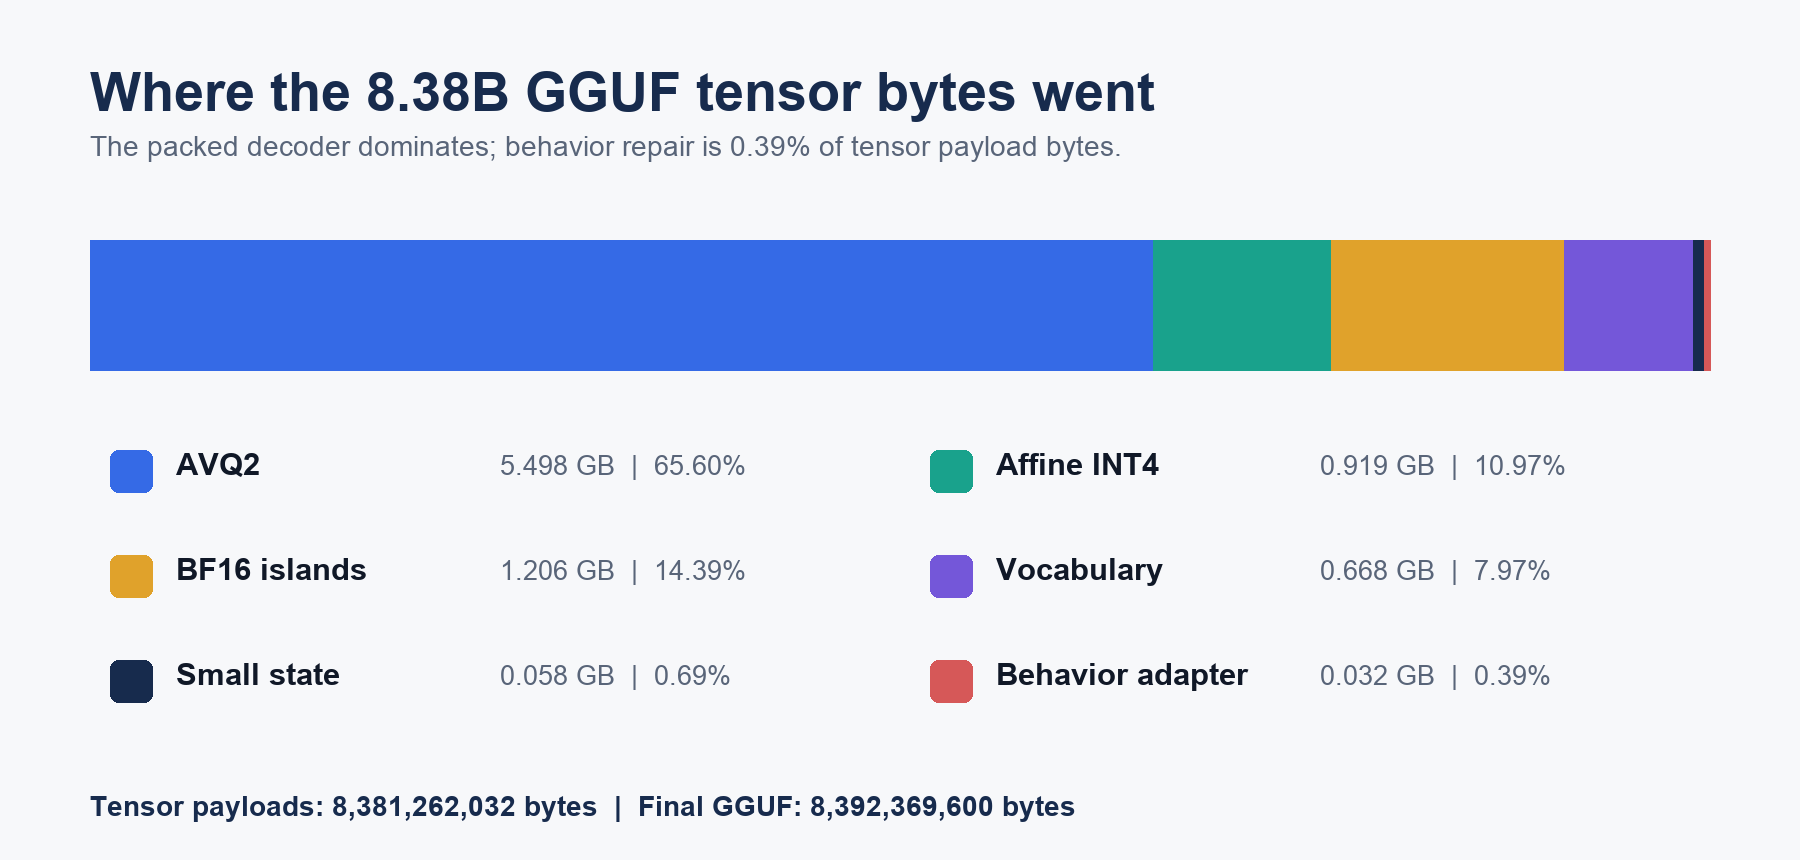
\includegraphics[width=\columnwidth]{figures/byte-allocation.png}
\caption{Physical tensor allocation in the final GGUF.}
\end{figure}

\section{Artifact proof}

The standalone loader meta-instantiates the text architecture, installs compact state and packed operators, attaches both corrections, and asserts that no compatible dense decoder matrix survives. The exporter byte-verified every tensor payload and reported no unsupported representation or runtime gap.

The exact GGUF generated through native CUDA and Metal. Three full-offload \code{llama-bench} runs on an RTX PRO 6000 Blackwell measured $84.70\pm0.37$ prompt tokens/s and $43.16\pm0.29$ generated tokens/s for a 512-token prompt and 128-token generation. An Apple M2 16 GB compatibility smoke measured 2.30 prompt tokens/s and 2.48 generated tokens/s. These are measurements of two systems, not a general performance model.

\section{Fresh release gate}

The release gate was authored after the compression, adapter, rescued rows, and byte allocation were frozen. It contains 100 turns, 20 each for single, parallel, sequential, parallel-multiple, and abstention behavior, using a new first-party tool namespace. Mechanical QA checked schema validity, duplicate IDs, parsing, and overlap.

The teacher solved 90/100. Its ten misses were all parallel-multiple. The compact artifact solved 83/100 and retained 83/90 teacher-correct turns. All generations stopped. Seven outputs were malformed, all in parallel-multiple. Manual inspection found fluent over-abstention rather than parser false negatives.

\begin{table}[t]
\centering
\small
\caption{Conditional retention on teacher-correct turns.}
\begin{tabular}{lrr}
\toprule
Category & Retained & Rate \\
\midrule
Single & 20/20 & 100\% \\
Parallel & 20/20 & 100\% \\
Sequential & 20/20 & 100\% \\
Parallel-multiple & 3/10 & 30\% \\
Abstention & 20/20 & 100\% \\
\midrule
Overall & 83/90 & 92.2\% \\
\bottomrule
\end{tabular}
\end{table}

The result passes the predeclared 90\% overall rule and fails the 90\% per-category rule. We report both. The gate is a private contract-retention test, not a frontier benchmark.

\section{What is new, and what is not}

We did not invent GPTQ-style curvature, SparseGPT, affine-lattice vector quantization, Hadamard incoherence, LDLQ, mixed precision, LoRA, or low-rank error correction. The AVQ2 core is closest to UniSVQ and related vector methods \cite{unisvq,qtip,vptq}. The curvature and propagated-error view follows GPTQ and SparseGPT \cite{gptq,sparsegpt}. The low-rank pieces follow established quantization-error and parameter-efficient adaptation work \cite{lqlora,qlora}.

The BTL contribution is the cookbook that joined those components and decided between them using emitted behavior. Specifically: packed-prefix bisection, behavior-proven precision promotion, rejection of a reconstruction stage that improved the wrong objective, training the correction against the final packed graph, separate treatment of serialization-sensitive vocabulary rows, exact physical byte exchange, and a sealed artifact-level gate. We believe that combination and decision protocol are novel. Each mathematical primitive is attributed to its prior method family.

\section{Limitations}

The private gate is small and synthetic. Parallel-multiple has only ten teacher-correct cases, and compact retention there is poor. The compact artifact has not yet established public coding-benchmark retention relative to the teacher. Long-context behavior was not validated uniformly across the 262K architectural window. Only one Qwen-derived 27B checkpoint was compressed, so the precision map may not transfer. The released GGUF requires the BTL packed backend; stock Ollama and LM Studio engines do not decode AVQ2 directly. Mobile performance, energy use, batching, and broad GPU coverage remain unmeasured.

\section{Reproduction recipe}

For clarity, the executed process is listed without narrative:

\begin{enumerate}
\item Freeze the base revision, adapter checksum, tokenizer, evaluator, and byte ceiling.
\item Create family-disjoint calibration, validation, development, and sealed release splits.
\item Balance the agent half across action shapes and abstention; mix it 1:1 with broad code/general data.
\item Starting at layer 0, replay calibration through the already packed prefix.
\item Accumulate FP64 input second moments for the current layer.
\item Apply seeded 128-wide block-Hadamard transforms.
\item Fit four-weight affine codes with block-LDLQ, scale search $\{0.8,1.0,1.2\}$, and ten refinement passes.
\item Quantize the three gated-MLP projections as one functional unit when a failure localizes there.
\item Pack codes and metadata; verify unpacked hard-graph parity.
\item Install the layer, checksum it, and capture the next layer from the real packed prefix.
\item Gate prefixes at short intervals. Use KL and reconstruction error only to locate suspects.
\item At the first behavioral flip, compare module and module-group overrides on the identical cases.
\item Promote only the smallest intervention that restores emitted behavior, and count its bytes.
\item Continue to all 64 layers using restart-safe manifests.
\item Freeze the decoder. Train the bounded rank-8 correction on the exact packed graph.
\item Quantize the embedding; rescue a fixed budget of structural and frequent rows.
\item Quantize the head and fit the activation-weighted rank-32 residual.
\item Solve the complete byte ledger. If over budget, demote only previously measured islands.
\item Export one native file, byte-verify every payload, and reject any dense fallback.
\item Open a newly authored sealed gate and report every behavior family separately.
\end{enumerate}

\section{Conclusion}

The project did not produce a universal two-bit recipe. It produced one fully accounted artifact and a record of how we reached it. Scalar sub-two-bit models could look competent under token metrics while being unable to act. Vector coding made the core viable, but the shippable result depended on debugging the packed computation at the behavior boundary, spending precision only where an intervention worked, and counting the entire file rather than the convenient part of it.

The final claim is intentionally limited: BTL-3 Compact is an 8.39 GB native text model that retained 83 of 90 teacher-correct turns on the stated tool-contract gate. The weak parallel-multiple result remains visible. That is a more useful result than a larger, cleaner number attached to the wrong metric.

\balance
\begin{thebibliography}{12}
\bibitem{gptq} E. Frantar et al. GPTQ: Accurate Post-Training Quantization for Generative Pre-trained Transformers. arXiv:2210.17323, 2022.
\bibitem{sparsegpt} E. Frantar and D. Alistarh. SparseGPT: Massive Language Models Can Be Accurately Pruned in One-Shot. arXiv:2301.00774, 2023.
\bibitem{aqlm} E. Egiazarian et al. Extreme Compression of Large Language Models via Additive Quantization. arXiv:2401.06118, 2024.
\bibitem{pvtuning} V. Malinovskii et al. PV-Tuning: Beyond Straight-Through Estimation for Extreme LLM Compression. arXiv:2405.14852, 2024.
\bibitem{qtip} A. Tseng et al. QTIP: Quantization with Trellises and Incoherence Processing. arXiv:2406.11235, 2024.
\bibitem{vptq} S. Liu et al. VPTQ: Extreme Low-bit Vector Post-Training Quantization for Large Language Models. arXiv:2409.17066, 2024.
\bibitem{unisvq} Z. Wang et al. UniSVQ: 2-bit Unified Scalar-Vector Quantization. arXiv:2606.10520, 2026.
\bibitem{yaqa} A. Tseng et al. Model-Preserving Adaptive Rounding. arXiv:2505.22988, 2025.
\bibitem{lqlora} H. Guo et al. LQ-LoRA: Low-rank Plus Quantized Matrix Decomposition for Efficient Language Model Finetuning. arXiv:2311.12023, 2023.
\bibitem{qlora} T. Dettmers et al. QLoRA: Efficient Finetuning of Quantized LLMs. arXiv:2305.14314, 2023.
\bibitem{paretoq} S. Liu et al. ParetoQ: Scaling Laws in Extremely Low-bit LLM Quantization. arXiv:2502.02631, 2025.
\bibitem{bonsai} PrismML. Bonsai 27B technical report and model cards, 2026.
\end{thebibliography}

\end{document}
